\section{Radiation Pressure}

Further Reading: Draine 41.7 


\begin{equation}
    P_{rad} = \frac{4\pi}{3}I_{\lambda}d_{\lambda}
\end{equation}
\begin{equation}
    P_{rad} = \int \frac{4 \pi}{3} \sigma T^{4}
\end{equation}
Radiation Pressure as a function intensity, and then of time. 


\section{Plane Parallel Atmosphere}

Definition: A \underline{plane parallel} atmosphere is one where the physical properties only change in the z-direction.\newline
Definition: A \underline{grey atmosphere} is one where $\tau$ is not dependent on $\nu$. \newline
Thus, because $S_{\nu}$ is proportional $ds$, we can also say that $S_{\nu}$ is proportional to $d\tau$ (since $d\tau=\kappa\rho ds$)

\begin{equation}
    S_{\nu} \propto d\tau_{\nu}
\end{equation}

\begin{figure}[h]
    \centering
    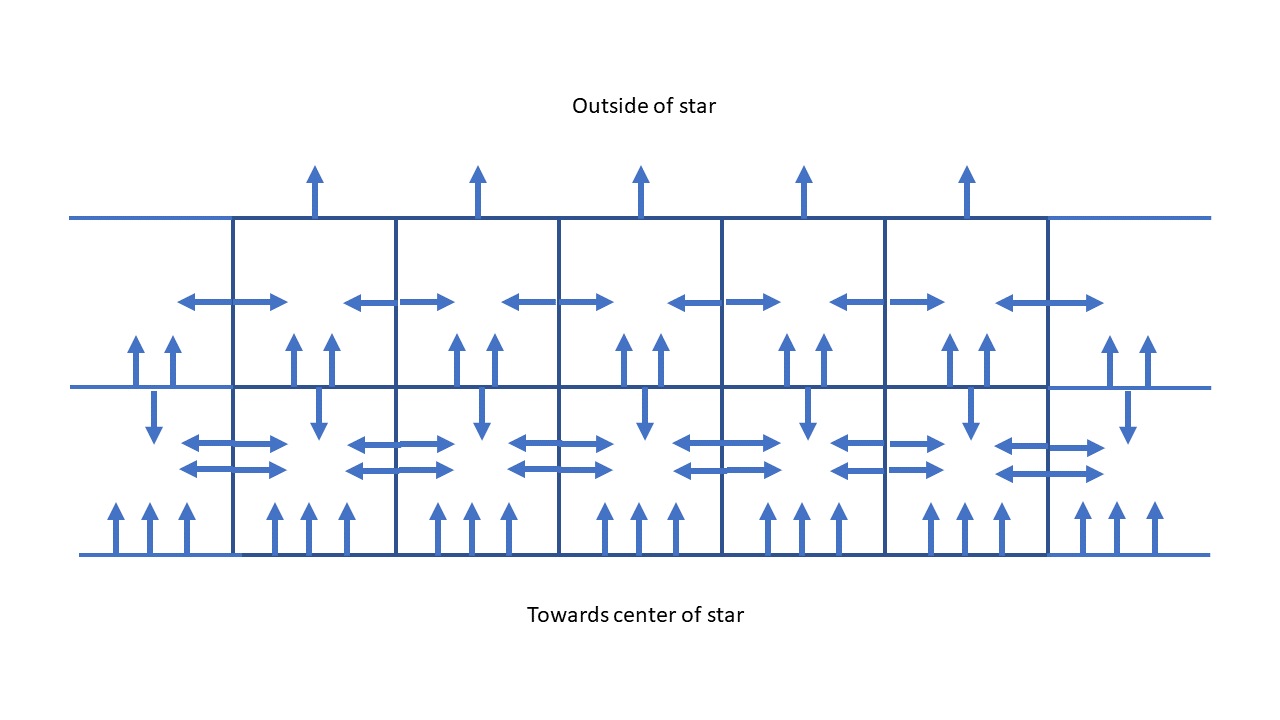
\includegraphics[width=0.7\columnwidth]{radProc_parallel_gmm.png}
    \caption{In order to have emission, there must be more photons etc deeper within the star.}
\end{figure}


\section{Eddington-Barbier Relation}

Approximation: near top of atmosphere ($\tau$<<1),Taylor expand Source function:
\begin{equation}
    S(\tau_{\lambda},v) \approx S_{\lambda}(0) + S_{\lambda}(0) \tau_{\lambda} = a + b \tau_{\lambda}

\end{equation}
Substitute into:

\begin{equation}
    I = \int_{0}^{\infty} S_v T_v e^{-T_v/\mu} d\tau / \mu
\end{equation}

\begin{equation}
    I_{\labmda}(\tau_{\lambda} = 0, \mu > 0) = a + b\mu
\end{equation}

\begin{equation}
    I_{\labmda}(\tau_{\lambda} = 0, \mu > 0) = S_{\lambda}(\tau_{\lambda}= \mu)
\end{equation}

\begin{equation}
    \tau_{\lambda} = \tau_{\lambda} sec \theta = \tau_{\lambda}\mu 
\end{equation}


So intensity I$_{\labmda}$ tells us S$_v$ as a function of $\mu$
\begin{equation}
    I_{\lambda}(τ_{\lambda} = 0, \mu > 0) = S_{\lambda}(τ_{\lambda} = 1)
\end{equation}





\section{Limb Darkening}
Start with the equation of radiative transfer:
\begin{equation}
    \frac{d I_{\nu}}{d \tau_{\nu}}=-I_{\nu} + S_{\nu}
\end{equation}
Multiplying both sides with $e^{-\tau_{\nu}}$ and get:
\begin{equation}
   e^{-\tau_{\nu}} \cdot \frac{d I_{\nu}}{d \tau_{\nu}}=(-I_{\nu} + S_{\nu}) \cdot e^{-\tau_{\nu}}
\end{equation}
Integrate by parts:
\begin{equation}
   \frac{d}{d\tau_{\nu} } (I_{\nu} \cdot e^{-\tau_{\nu}})= -S_{\nu} \cdot  e^{-\tau_{\nu}}
\end{equation}
Integrate w.r.t $\tau_{\nu}$ and get:
\begin{equation}
   I_{\nu}=I_{\nu}(0)e^{-\tau_{\nu}}+\int_{0}^{\tau_{\nu}} S_{\nu} e^{-(\tau_{\nu}\prime-\tau_{\nu})} d\tau_{\nu}\prime
\end{equation}
Assuming that we are all the way into the core, i.e. $\tau_{\nu} \rightarrow \infty$, only the second term would contribute:
\begin{equation}
   I_{\nu}=\int_{0}^{\tau_{\nu}} S_{\nu} e^{-(\tau_{\nu}\prime-\tau_{\nu})} d\tau_{\nu}\prime
\end{equation}
Assuming plane parallel atmosphere:
\begin{equation}
\tau_{\nu}\prime-\tau_{\nu} = \tau_{\nu} \cdot \sec(\theta)
\end{equation}
Plug this in and use the fact that the source function is a linear function of $\tau_{\nu}$ because of isotropic nature of the radiation:
\begin{equation}
   I_{\nu}=\int_{0}^{\infty} (a+b\cdot\tau_{\nu} ) e^{-\tau_{\nu} \cdot \sec(\theta)} \sec(\theta) d\tau_{\nu}
\end{equation}
Evaluate the above integral and get:
\begin{equation}
   I_{\nu}=a_{\nu} + b_{\nu} \cdot \cos(\theta)
   \label{eq:1}
\end{equation}

For the case of the Sun, we have derived the formula for the source funtion:
\begin{equation}
   S_{\nu}=\langle I_{\nu} \rangle =\frac{3 \sigma}{4 \pi} T_{e}^{4} \cdot (\tau_{\nu}+\frac{2}{3}) = a + b\cdot \tau_{\nu}
\end{equation}
Comparing the coefficients, we get the value for $a_{\nu}$ and $b_{\nu}$:
\begin{equation}
   a_{\nu}=\frac{\sigma}{2\pi}\cdot T_{e}^{4}
\end{equation}
\begin{equation}
   b_{\nu}=\frac{\sigma}{4\pi}\cdot T_{e}^{4}
\end{equation}
Put there values into \eqref{eq:1} and we can find the ratio of the specific intensity at angle $\theta$ and angle zero is:
\begin{equation}
   \frac{I_{\nu}(\theta)}{I_{\nu}(0)}=\frac{a_{\nu}+b_{\nu}\cos(\theta)}{a_{\nu}+b_{\nu}}=\frac{2}{5}+\frac{3}{5}\cdot \cos(\theta)
\end{equation}



\section{Curve of Growth}\label{sec:growthcurve}

\fbox{\parbox{\textwidth}{TL;DR How do the equivalent width of absorption lines evolve with increasing number of absorbers $N$?
\begin{itemize}
    \item Weak lines: Doppler broadening, $EW\propto N$
    \item Saturated lines: Doppler broadening, but only in the wings, $EW \propto \sqrt{ln(N)}$
    \item Strong lines: Lorentzian profile begins to dominate due to collisional broadening, $EW \propto \sqrt{N}$
\end{itemize}}}
\begin{figure}
    \centering
    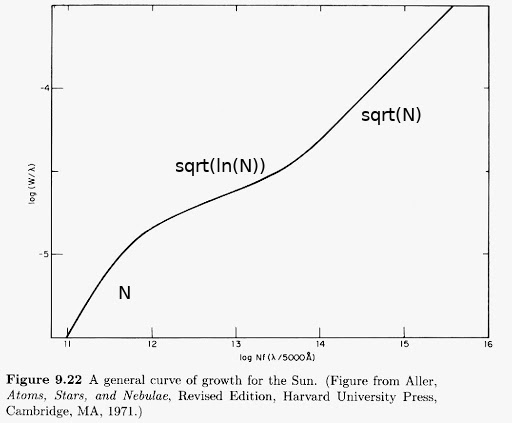
\includegraphics[scale=0.6]{growthcurve.jpg}
    \caption{A labeled, graphical representation of the curve of growth for equivalent widths of absorption lines in the Sun.}
    \label{fig:growth_curve}
\end{figure}

\textbf{More detail:}\newline
Consider an absorption line surrounded by continuum emission at intensity $I_{0}$ and a (reduced) minimum intensity of $I_{\nu}$. Its equivalent width, a measure of the total amount of radiation absorbed in a particular line, is given by the integral of the absorption depth $D$:
\begin{equation}
    EW = \sum_{\nu}D d\nu = D_{\rm max}\sum_{\nu}(1-I/I_{0})d\nu=\sum_{\nu}(1-e^{-\tau})d\nu
\end{equation}
where $\tau$ is the optical depth of the absorber and $D_{\rm  max}$ is the maximum depth of the line. A fundamental question here is, then: How does the equivalent width of an absorption line change as more atoms contribute to it (i.e. the number of absorbers $N$ increases), and what forms can these contributions take?\newline
For a small amount of absorbing atoms (i.e. low density, weak lines), the dominant physical process governing line width is Doppler broadening. Taking the low density of the absorber to mean $\tau \ll 1$, the absorption depth $(1-e^{-\tau})$ is approximately $\tau$. The optical depth itself follows a Voigt profile (see \ref{sec:line_profile}), with a Gaussian center due to random motions causing red/blueshift but Lorentzian wings due to collisions; however, since Doppler broadening dominates in this low-optical-depth regime, we can assume it instead follows a completely Gaussian profile around the central line frequency. When integrated to give the EW, this gives \framebox{$EW \propto N$}. (Maybe a quicker way to conceive of this is as follows: since $\tau=\kappa\rho s$ for some assumptions about the cloud, the optical depth varies linearly with density, and the equivalent width varies linearly with the optical depth while it is low.)\newline
However, increasing the number of absorbers will eventually end in the complete absorption of the initial intensity. At this point ($\tau\approx 5$), the EW cannot increase by decreasing intensity at the exact frequency of the line, so it must come from the wings of the Gaussian instead, as the optical depth is still not high enough for collisional processes (and therefore, the Lorentzian wings) to significantly matter (although they will in a little bit.) What increases there are in the EW, then, are much slower: to a good approximation, \framebox{$EW \propto \sqrt{ln(N)}$}.\newline
As the density continues to rise, collisions will become increasingly important; the resulting distribution of velocities will lead to an optical depth that falls off as $(\nu-\nu_{0})^{-2}$ for $\nu$ sufficiently far away from the line frequency $\nu_{0}$, which at this point are the only unsaturated regions. This shape is clearly not a Gaussian, so it follows that the EW will evolve differently: substituting the Lorentzian profile into the EW integral will yield \framebox{$EW \propto \sqrt{N}$}.